\section{Durchführung}
\label{sec:Durchführung}

Es wird durch ein schwenkbares Photoelement die Intensität eines Laser, der von einer Si-Oberfläche reflektierten Strahlung gemessen \autoref{fig:aufbau}.
Zwischen dem Laser und der Si-Oberfläche wird zusätzlich ein Polfilter platziert, damit das senkrecht vom parallel polarisierten Licht getrennt werden kann.
Die Si-Oberfläche ist auf einer Drehscheibe montiert, damit der Einfallswinkel des Laserlichts variiert werden kann. Das Photoelement muss immer so ausgerichtet werden, dass das Licht direkt in die Öffung des Photoelements fällt.
Ein Amperemeter misst den Strom, welcher durch den Laser im Photoelement erzeugt wird. Der gemessene Strom ist proportional zur Intensität, also zum Quadrat der Feldstärke.
Zunächst wird der Nullstrom gemessen, also die direkte Leistung des Lasers.

\begin{figure}[H]
    \centering
    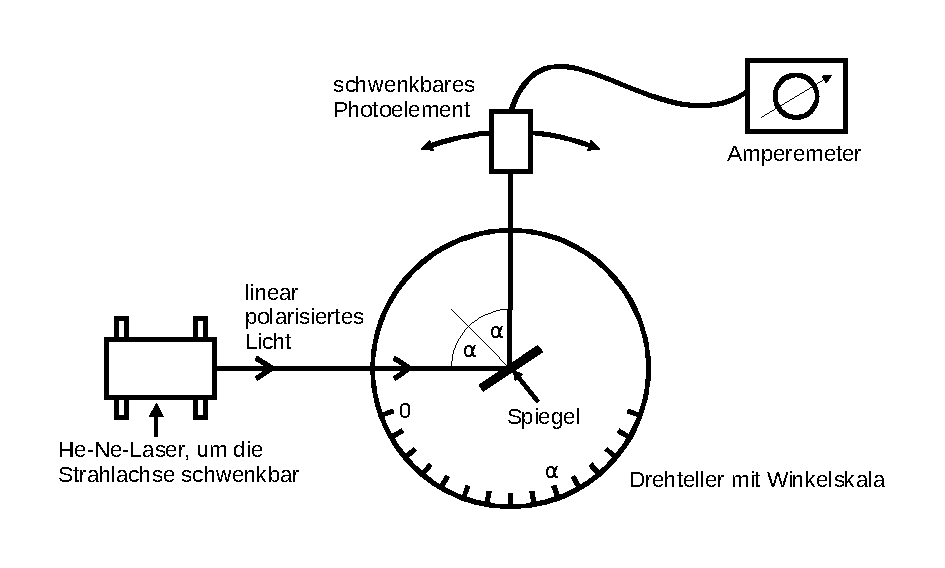
\includegraphics{Aufbau.pdf}
    \caption{Schematische Darstellung der Messapperatur \cite{ap01}.}
    \label{fig:aufbau}
\end{figure}
